\documentclass[10pt,twocolumn,letterpaper]{article}

\usepackage{cvpr}
\usepackage{times}
\usepackage{epsfig}
\usepackage{graphicx}
\usepackage{amsmath}
\usepackage{amssymb}
\usepackage{xcolor}
% Include other packages here, before hyperref.

% If you comment hyperref and then uncomment it, you should delete
% egpaper.aux before re-running latex.  (Or just hit 'q' on the first latex
% run, let it finish, and you should be clear).
\usepackage[breaklinks=true,bookmarks=false]{hyperref}

\cvprfinalcopy % *** Uncomment this line for the final submission

\def\cvprPaperID{****} % *** Enter the CVPR Paper ID here
\def\httilde{\mbox{\tt\raisebox{-.5ex}{\symbol{126}}}}

% Pages are numbered in submission mode, and unnumbered in camera-ready
%\ifcvprfinal\pagestyle{empty}\fi
\setcounter{page}{4321}
\begin{document}

%%%%%%%%% TITLE
\title{Facial expression recognition application using CNNs}

\author{
Peagno Eleonora \\\normalsize 1237035\\
%{\tt\small }
% For a paper whose authors are all at the same institution,
% omit the following lines up until the closing ``}''.
% Additional authors and addresses can be added with ``\and'',
% just like the second author.
% To save space, use either the email address or home page, not both
\and
Peron Giovanni \\\normalsize 1237783\\
%{\tt\small secondauthor@i2.org}
\and
Rossi Daniel \\\normalsize 1211017\\
%{\tt\small secondauthor@i2.org}
}

\maketitle
%\thispagestyle{empty}

%%%%%%%%% ABSTRACT
\begin{abstract}
   %The ABSTRACT is to be in fully-justified italicized text, at the top
   %of the left-hand column, below the author and affiliation
   %information. Use the word ``Abstract'' as the title, in 12-point
   %Times, boldface type, centered relative to the column, initially
   %capitalized. The abstract is to be in 10-point, single-spaced type.
   %Leave two blank lines after the Abstract, then begin the main text.
   %Abstract should be no longer than 300 words.
   The facial expression recognition is a challenging task in machine learning field, 
   and there is an active research on this topic. Being able to make a machine understand 
   the human emotions is a fascinating goal.
   The purpose of this report is to exploit all the topics studied during 
   the Vision and Cognitive Services course and others like Machine Learning and Deep Learning
   in order to implement a system able to predict human emotions.
   We will describe how we realized this system specifying all the steps performed,
   from the first CNN we tried to the final model we obtained. 
   We will illustrate all the procedure we used trying to achieve better results.
   Our target was not very high since this is a challenging task as we said, however
   with our final model we arrived to a predition accuracy of \textbf{\textcolor{red}{...}} that is better than the human accuracy.
   Finally using this model we reached our goals implementing a nice application.
\end{abstract}

%%%%%%%%% BODY TEXT
\section{Introduction}
   Facial expressions recognition (FER) is an interesting and a challenging problem 
   in machine learning field. It is also a task that can be applied in many important applications.
   Facial expressions have an important role in every human interaction so having a machine able to 
   recognize and understand human expressions automatically can be very useful
   in many existing and novel fields. [2.pdf Cap 4 Opportunities]
   \\One of these fields is behaviomedics that are systems which exploit automatic analysis of affective and social signals 
   to aid diagnosis, monitoring and treating medical condition that alter behavior.
   Facial expression recognition can be also use in data analytics field for example to understand 
   emotions of people that are looking at ads or political debate and make statistics related to people's preferences. 
   Another application field for Facial expression recognition is human-computer interaction, understanding human emotions 
   would make the attitude of systems like vocal assistants or robots much closer to the way that humans interact with each other.
   Recognizing expressions could also be useful to improve the identification of micro facial expressions which can be used in 
   deceit detection applications.
   Due to all these possible applications, facial expressions recognition is widely studied also because recognizing 
   human expressions in natural condition environment is a very challenging task.
   With this project we aim to build a facial expressions classifier able to reach the human accuracy on this task, 
   that with the dataset used is 65.5\% [3]. 
   The main idea was focusing mostly on study different types of model in order to understand a good way to achieve valid outcomes.
   For this reason all preprocessing techniques that can be applied to the input data for improving classification results were not be consider.
   Dataset
   Results 




\section{Related Work}
\section{Dataset}
\section{Method}
\section{Experiments}
\section{Conclusion}



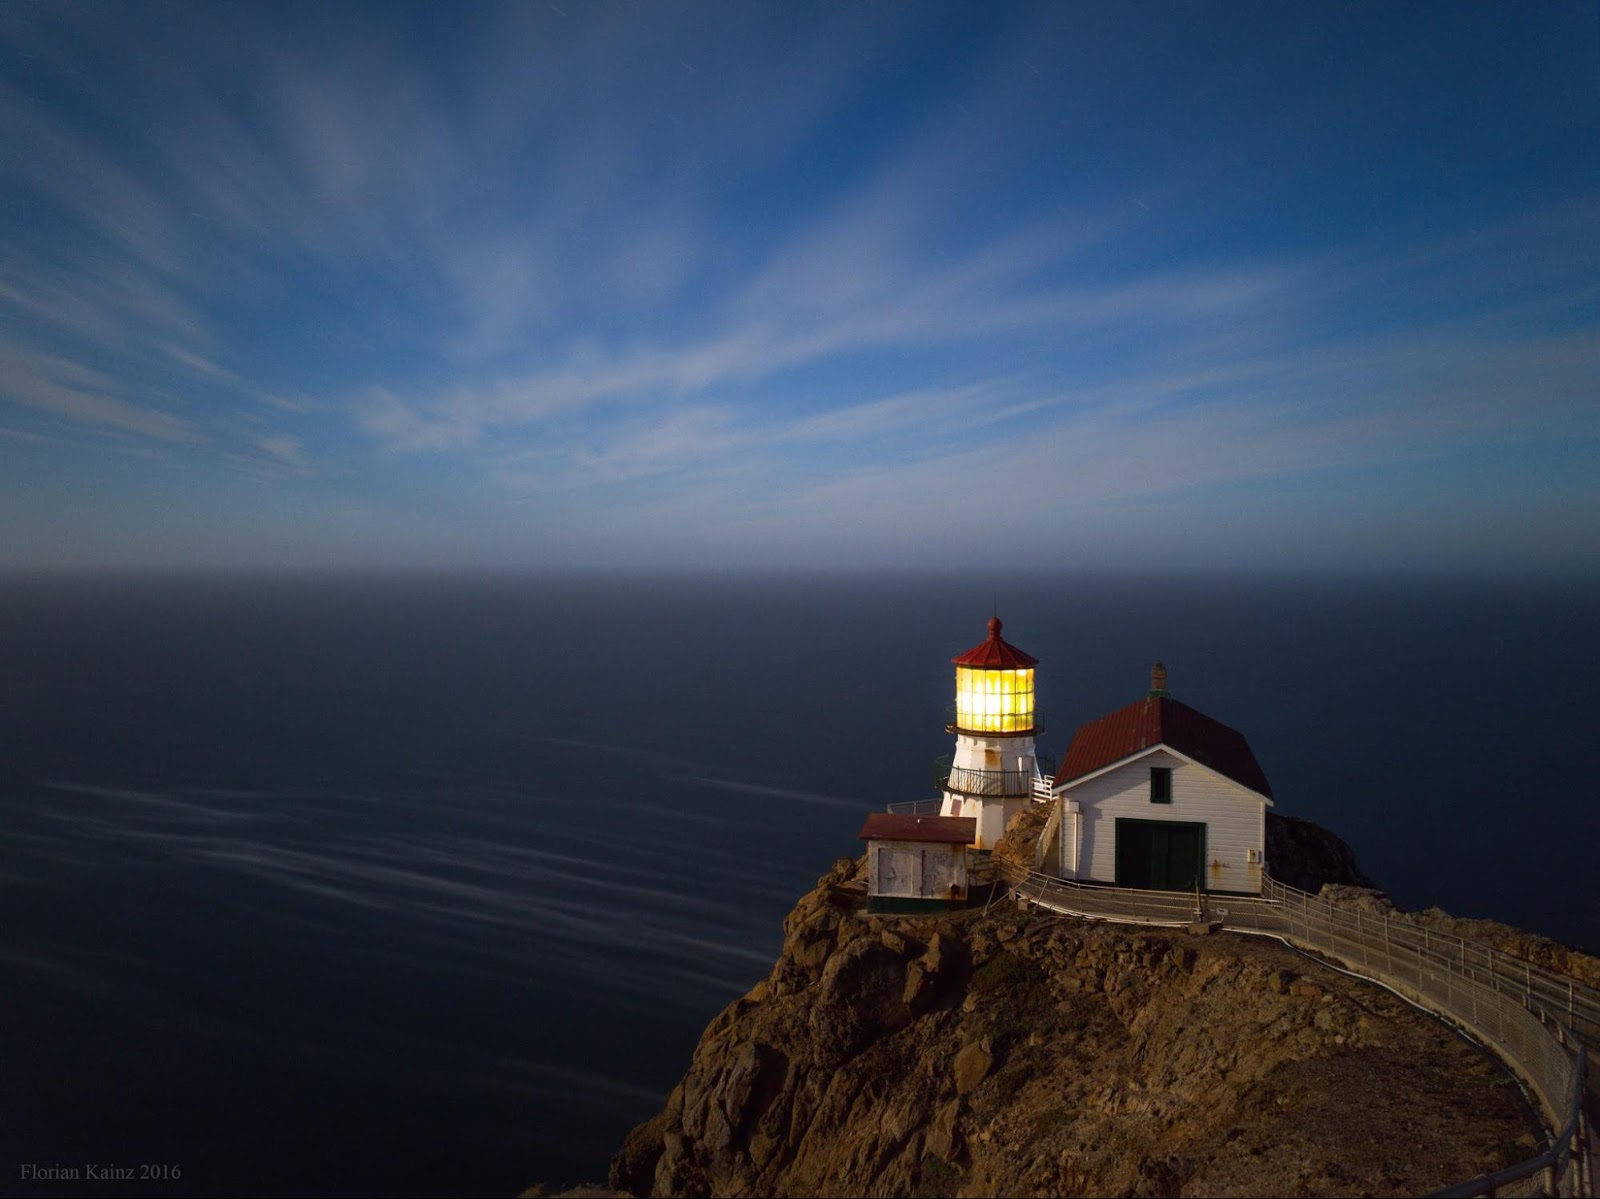
\includegraphics[width=0.8\linewidth]{./immagini/app-google-foto-notte-5.jpg}



{\small
\bibliographystyle{ieee_fullname}
\bibliography{egbib}
}

\end{document}
